\documentclass[11pt,a4paper]{article}\usepackage[utf8]{inputenc}

\usepackage[T1]{fontenc}
\usepackage{tgpagella}
\usepackage[spanish]{babel}
\usepackage{geometry}
\usepackage{graphicx}
\usepackage{booktabs}
\usepackage{array}
\usepackage{xcolor}
\usepackage{titlesec}
\usepackage{fancyhdr}
\usepackage[parfill]{parskip}
\usepackage[expansion=false]{microtype}
\usepackage{hyperref}
\usepackage{setspace}
\usepackage{needspace}

\geometry{top=3.0cm,bottom=3.0cm,left=3.5cm,right=3.5cm}
\setlength{\parskip}{0.65em}
\setlength{\parindent}{0em}

\definecolor{azulai}{RGB}{30,80,140}
\definecolor{doradoai}{RGB}{140,90,0}
\definecolor{grisai}{RGB}{70,70,70}

\titleformat{\section}{\Large\bfseries\color{azulai}}{}{0em}{}[{\color{azulai}\titlerule[0.5pt]\nopagebreak[4]}]
\titlespacing*{\section}{0pt}{1.8em}{0.8em}
\titleformat{\subsection}{\large\bfseries\color{doradoai}}{}{0em}{}[{\nopagebreak[4]}]
\titlespacing*{\subsection}{0pt}{1.4em}{0.5em}
\titleformat{\subsubsection}{\normalsize\bfseries\color{grisai}}{}{0em}{}[{\nopagebreak[4]}]
\titlespacing*{\subsubsection}{0pt}{1.0em}{0.3em}

\pagestyle{fancy}\fancyhf{}
\rhead{\textcolor{grisai}{\small Nieves Arrarás — Arquitectura Interna}}
\lhead{\textcolor{grisai}{\small Carta Natal Completa}}
\cfoot{\textcolor{grisai}{\small\thepage}}
\renewcommand{\headrulewidth}{0.3pt}

\hypersetup{colorlinks=true,linkcolor=azulai,urlcolor=azulai}
\setstretch{1.45}
\tolerance=1500
\emergencystretch=4em

\begin{document}

% ── Portada ──────────────────────────────────────────────────────────────────
\begin{titlepage}
  \centering
  \vspace*{1.5cm}
  {\Huge\bfseries\color{azulai} Carta Natal Completa}\\[0.5cm]
  {\large\color{grisai} Arquitectura Interna}\\[0.3cm]
  {\small\itshape\color{grisai} Un método para sostener cuerpo, energía y vida con coherencia}\\[2cm]
  {\huge\color{doradoai} Nieves Arrarás}\\[1.5cm]
  {\Large 01/12/1948 \quad 01:20}\\[0.3cm]
  {\Large Pamplona, España}\\[0.3cm]
  {\normalsize Lat: 42.8157° \quad Lon: -1.6522° \quad UTC+01:00}\\[0.3cm]
  {\normalsize Ascendente: Virgo 16°53' \quad
    MC: Géminis 14°27'}\\[2.5cm]
  \vfill
  {\small Generado el 13/05/2026}
\end{titlepage}

\tableofcontents
\newpage

% ── Rueda ─────────────────────────────────────────────────────────────────────
\section{Carta Natal}
\begin{figure}[h!]
  \centering
  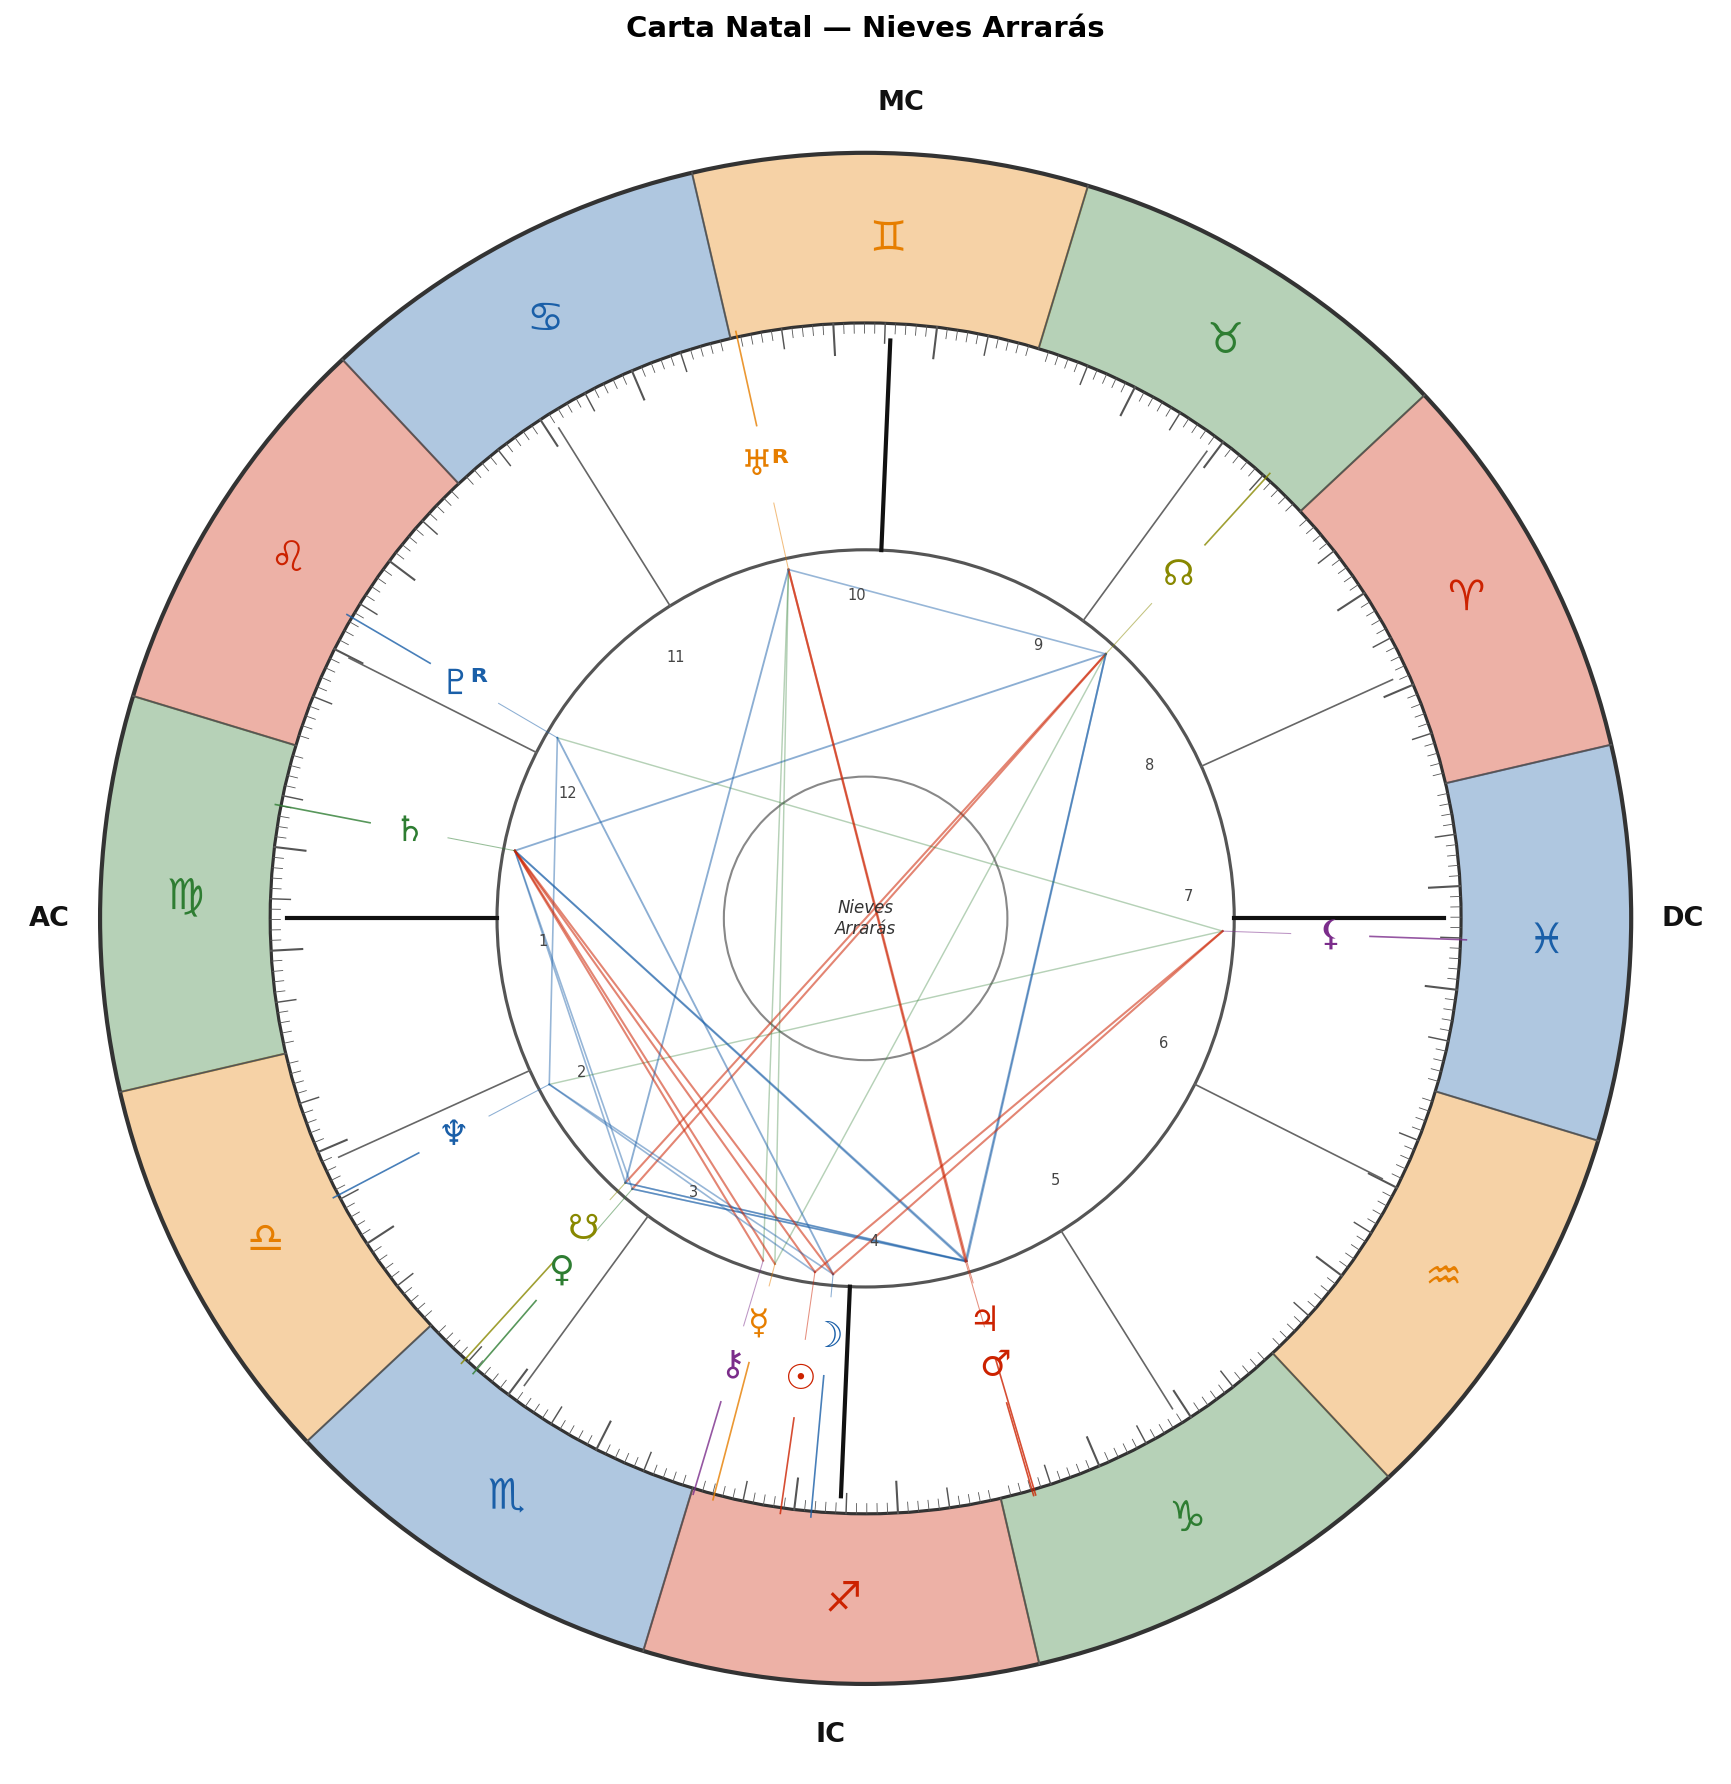
\includegraphics[width=0.90\textwidth]{Nieves_Arrarás_AI_rueda.png}
  \caption{Carta natal de Nieves Arrarás — 01/12/1948 01:20 — Pamplona, España}
\end{figure}

\newpage

% ── Tabla de posiciones ───────────────────────────────────────────────────────
\section{Posiciones Planetarias}

\begin{center}
\begin{tabular}{llrrlll}
  \toprule
  \textbf{Planeta} & \textbf{Signo} & \textbf{Grado} & \textbf{Casa} &
  \textbf{Elemento} & \textbf{R} \\
  \midrule
  Sol & Sagitario & 8°44' & 3 & Fuego &  \\
  Luna & Sagitario & 11°39' & 3 & Fuego &  \\
  Mercurio & Sagitario & 2°10' & 3 & Fuego &  \\
  Venus & Escorpio & 6°07' & 2 & Agua &  \\
  Marte & Capricornio & 3°07' & 4 & Tierra &  \\
  Júpiter & Capricornio & 3°19' & 4 & Tierra &  \\
  Saturno & Virgo & 5°58' & 12 & Tierra &  \\
  Urano & Géminis & 29°21' & 10 & Aire & R \\
  Neptuno & Libra & 14°35' & 2 & Aire &  \\
  Plutón & Leo & 16°31' & 11 & Fuego & R \\
  Quirón & Sagitario & 0°13' & 3 & Fuego &  \\
  Lilith & Piscis & 14°50' & 6 & Agua &  \\
  Nodo Norte & Tauro & 4°38' & 8 & Tierra &  \\
  Nodo Sur & Escorpio & 4°38' & 2 & Agua &  \\
  \bottomrule
\end{tabular}
\end{center}

\vspace{0.5cm}
\begin{itemize}
  \item \textbf{Ascendente:} Virgo 16°53'
  \item \textbf{Medio Cielo:} Géminis 14°27'
\end{itemize}

\newpage

% ── Interpretación ────────────────────────────────────────────────────────────
\section{Interpretación — Arquitectura Interna}

\begin{center}
{\small\itshape
No se trata de definirte. Se trata de observar cómo se organiza tu energía,\
dónde puedes perder equilibrio y qué apoyos te ayudan a sostenerte.
}
\end{center}

\vspace{0.5cm}

\subsection{1. Visión General}

Tu carta muestra la siguiente distribución de elementos: Fuego 7.5, Tierra 5.5, Aire 2, Agua 1.5. Fuego (vitalidad, iniciativa, necesidad de sentido y movimiento hacia la acción) y Tierra (arraigo en lo concreto, estructura material, ritmo sostenido y contacto con el cuerpo): ahí está el peso de tu carta. Es el registro desde el que tu energía se activa con más fluidez y sin esfuerzo consciente. Aire (desapego, análisis, pensamiento relacional y capacidad de perspectiva) y Agua (profundidad emocional, capacidad de resonancia, sensibilidad abierta) está poco representado en tu carta. Ese territorio puede pedirte un esfuerzo consciente, especialmente cuando la presión sube. La mayoría de tus planetas están en signos mutables: hay facilidad para adaptarte, cambiar y responder a lo que ocurre alrededor. Sueles moverte bien cuando las situaciones evolucionan o requieren flexibilidad. La dificultad aparece cuando todo cambia al mismo tiempo y cuesta mantener una dirección estable durante suficiente tiempo. Tu Medio Cielo en Géminis: La comunicación, el aprendizaje y la capacidad de moverte entre distintos temas o personas. Funcionas bien en entornos donde la palabra, el intercambio y la circulación de ideas son importantes.

\subsection{2. Ejes Principales}

\subsubsection*{Sol en Sagitario — Casa 3}
Tu Sol en Sagitario necesita sentir que lo que haces tiene dirección y sentido para ti. Funcionas mejor cuando hay movimiento, aprendizaje o sensación de expansión. La capacidad de entusiasmarte y abrir perspectivas suele aparecer de forma natural. El riesgo aparece cuando la necesidad de avanzar hace difícil detenerte en lo cotidiano o sostener procesos lentos. En Casa 3, tu identidad se sostiene a través de la comunicación, el aprendizaje y el intercambio con tu entorno próximo. Necesitas que tus ideas tengan peso en los círculos cercanos. Pensar, hablar, preguntar y compartir ideas forma parte natural de cómo te orientas en el mundo.

\subsubsection*{Luna en Sagitario — Casa 3}
Tu Luna en Sagitario necesita movimiento, perspectiva y sentido. Cuando algo te afecta, te ayuda entender para qué sirve, hacia dónde te lleva o qué puedes hacer con ello. Si no encuentras una salida, el estado emocional puede convertirse en inquietud, impaciencia o necesidad de cambiar de escenario. El movimiento, el cambio de perspectiva y la sensación de amplitud te ayudan a recuperar estabilidad. En Casa 3, procesas las emociones a través del habla, el pensamiento y el intercambio cercano. Nombrar lo que sientes suele ayudarte a entenderlo mejor. El entorno próximo tiene peso emocional significativo.

\subsubsection*{Ascendente Virgo}
Tu Ascendente en Virgo hace que los demás te vean como una persona analítica, discreta y orientada al detalle. Observa y evalúa antes de participar. Puede haber una distancia inicial que no refleja la calidez que aparece cuando coges confianza. Su regente es Mercurio, en Sagitario y Casa 3. El Ascendente toma el tono de Sagitario: expansiva, entusiasta y orientada a ampliar horizontes. Esa energía opera principalmente desde la comunicación, el aprendizaje y el intercambio cercano.

\subsubsection*{Grados finales de signo}
Los grados finales de signo muestran funciones que están cerca de un punto de cierre, maduración o cambio de modo. No se interpretan como destino ni como algo negativo, sino como zonas donde la energía del signo aparece muy concentrada. Puede haber más intensidad, menos margen para funcionar de forma automática y una sensación interna de que una forma antigua de responder ya no se sostiene igual.

En esta carta hay posiciones en grado anarético. El grado 29 suele señalar una función llevada al límite de su signo: hay mucha experiencia acumulada, pero también una presión interna para dejar de repetir el patrón de forma inconsciente.

Urano en Géminis 29°21', Casa 10 aparece en grado anarético. La necesidad de libertad, cambio y ruptura de patrones aparece en un punto de máxima intensidad. Puede haber muy poca tolerancia a estructuras que se sienten cerradas, rígidas o demasiado previsibles. Cuando algo limita la autenticidad o el movimiento interno, la desconexión puede aparecer de forma repentina. El reto está en no convertir cada sensación de encierro en ruptura inmediata, sino en crear espacio antes de llegar al corte.

Cuando varios puntos de la carta se sitúan al final de signo, la interpretación necesita considerar que el sistema puede funcionar con menos margen de regulación automática. No significa que haya más dificultad, sino que esas zonas piden más cuerpo, más pausa y más consciencia antes de seguir respondiendo desde el patrón habitual.



\subsection{3. Organización de la Energía}

Tu Mercurio en Sagitario necesita entender el sentido general de las cosas. Piensas mejor cuando puedes ver el panorama completo y conectar una experiencia con algo más amplio. El riesgo aparece cuando el conjunto interesa tanto que los detalles quedan sin revisar. En Casa 3, Mercurio está en un territorio muy natural para él. Aprendes rápido a través de la conversación, el intercambio y el movimiento cercano. La curiosidad y la necesidad de entender lo que ocurre alrededor suelen estar muy activas. Tu Venus en Escorpio se vincula con intensidad y necesidad de confianza real. No te alimentan los vínculos superficiales cuando algo importa de verdad. El riesgo aparece cuando el miedo a perder o a quedar expuesto lleva a controlar más de lo necesario. En Casa 2, el afecto necesita estabilidad, continuidad y sensación de seguridad. Valoras mucho los gestos concretos, la presencia real y los vínculos que ayudan a construir algo sólido. Tu Marte en Capricornio actúa con estrategia, disciplina y orientación a largo plazo. Puede sostener esfuerzos prolongados cuando hay una meta clara. El riesgo aparece cuando la exigencia se vuelve demasiado dura y la acción pierde flexibilidad. En Casa 4, la acción está muy ligada al hogar, la intimidad y la necesidad de proteger tu espacio privado. Hay mucha fuerza disponible cuando se trata de defender lo que sientes como propio.

\subsection{4. Estructura y Tensión}

\subsubsection*{Concentración de energía}

Hay una concentración notable en Casa 3: Sol, Luna, Mercurio y Quirón. Cuando varios planetas ocupan la misma casa, esa área absorbe buena parte de la actividad vital. En esta carta, el foco de la comunicación, el aprendizaje y el entorno cercano funciona como núcleo central: ahí se acumula la presión, la demanda es mayor y también hay más recursos disponibles para operar. No es necesariamente un conflicto, pero sí un punto de alta intensidad sostenida.

También hay una concentración significativa en Casa 2: Venus, Neptuno y Nodo Sur. En este caso, el foco se desplaza hacia los recursos, la estabilidad y el valor propio. Es un ámbito donde la exigencia aumenta, donde se concentra parte de la presión y donde también existe capacidad real de sostener procesos importantes. Tampoco es en sí un problema, pero sí un área de intensidad mantenida.



Los aspectos aparecen organizados en dos niveles. Los aspectos exactos (orbe igual o menor a 1°) suelen sentirse de forma más inmediata y constante en la vida cotidiana. Los aspectos estructurales tienen un orbe más amplio, pero siguen describiendo dinámicas importantes que se repiten a lo largo de la vida.



\Needspace{8\baselineskip}
\subsubsection*{Aspectos exactos}
No aparecen aspectos exactos especialmente fuertes dentro del orbe definido para esta lectura. Eso no significa ausencia de tensión o profundidad, sino que gran parte de las dinámicas importantes de la carta se construyen de forma más amplia y progresiva. En este caso, cobran más importancia los aspectos estructurales y la combinación general de posiciones.

\Needspace{8\baselineskip}
\subsubsection*{Aspectos estructurales}
\Needspace{7\baselineskip}
\subsubsection*{Luna (Casa 3) cuadratura Saturno (Casa 12) --- orbe 5.69\textdegree}
La cuadratura Luna-Saturno marca una tensión entre lo que necesitas sentir y lo que te permites mostrar. Puede aparecer como contención emocional, dificultad para pedir apoyo o tendencia a exigirte estar bien antes de recibir cuidado. Desde fuera quizá pareces más fuerte de lo que realmente estás. La clave está en reconocer cuándo la exigencia interna te está costando más que la situación real.



\subsection{5. Sostén y Equilibrio}

Tu Quirón en Sagitario, Casa 3, señala una zona sensible relacionada con la confianza en tu visión, en tus ideas y en la posibilidad de avanzar con dirección propia. Puede que hayas sentido dudas sobre tu lugar, tus creencias o tu capacidad de encontrar un rumbo claro. Esto suele notarse especialmente en la comunicación, el aprendizaje y el entorno cercano. No significa que tengas límites en ese terreno, pero sí que probablemente necesites más tiempo, cuidado o consciencia para sentir estabilidad ahí.

\vspace{0.3cm}
Tu Nodo Sur en Escorpio, Casa 2, muestra una tendencia a moverte desde la intensidad constante, el control o la dificultad para soltar situaciones desgastadas, especialmente en el valor propio y la estabilidad material o emocional. Suele ser una forma de funcionar conocida o automática para ti. Tu Nodo Norte en Tauro, Casa 8, señala la necesidad de desarrollar construir estabilidad real, paciencia y una relación más sencilla con lo concreto, especialmente en la intimidad y las situaciones emocionalmente intensas. No se trata de rechazar lo anterior, sino de ampliar tu forma habitual de responder.

\vspace{0.3cm}


\subsection{6. Orientación}

\subsubsection*{Qué observar}
Tu Ascendente en Virgo describe la forma en que otras personas suelen percibirte al principio. Eso no siempre coincide con cómo vives las cosas internamente o con las tensiones más importantes de tu carta. Cuando hay demasiada distancia entre lo que muestras y lo que realmente te ocurre, aparece desgaste.

\subsubsection*{Qué puede desestabilizar}
Hay ciertas tensiones en tu carta que pueden activarse con bastante fuerza: Nodo Norte-Nodo Sur, Neptuno-Lilith, Urano-Quirón. Cuando varias coinciden al mismo tiempo, puede aparecer sensación de saturación, reacción excesiva o dificultad para mantener claridad.

\subsubsection*{Qué estructura y sostiene}
Tu Sol en Sagitario, Casa 3, muestra un terreno importante de estabilidad para ti. Cuando tu forma de actuar está alineada con lo que realmente valoras, suele aparecer más claridad y menos dispersión.

\subsubsection*{Orientación práctica}
Una orientación práctica: cuando todo se activa demasiado, no intentes resolverlo todo desde la cabeza. Empieza por algo pequeño y concreto que te devuelva presencia: caminar, ordenar una parte de tu espacio, cocinar, respirar con calma o hacer algo físico y sencillo. Muchas veces el cuerpo recupera claridad antes que la mente.

\vspace{1cm}
\begin{center}
{\small\itshape\color{grisai}
La astrología se usa aquí como lenguaje simbólico de observación, no como una definición de quién eres.\\
Esta interpretación es tu mapa de posibilidades, no tu destino fijo.
}
\end{center}

\end{document}
